%BAB-1 Laporan KP

\chapter{PENDAHULUAN}

\section{Latar Belakang Masalah}

	Perkembangan teknologi serta ilmu pengetahuan pada masa ke masa semakin berkembang. Perkembangan ini berjalan seiring dengan penelitian-penelitian di berbagai disiplin ilmu khususnya dalam bidang instrumentasi dan kendali. Hal ini dapat dilihat dari banyaknya penggunaan sistem instrumentasi dan kendali dalam dunia industri seperti pengguanaan robot dalam menyelesaiakan pekerjaan manusia.Untuk itu perancangan robot merupakan salah satu solusi untuk memenuhi tuntutan dalam membantu kebutuhan manusia.
	
	Pemilihan robot untuk menggantikan pekerjaan manusia tidak terlepas dengan berbagai kelebihannya. Robot dapat melakukan suatu pekerjaan yang sama dan berulang tanpa merasakan lelah seperti halnya manusia. Pekerjaan ini lah yang biasa ditemukan dalam bidang industri khususnya pada bagian produksi. Robot dengan sistem lengan robot (\emph {robot arm sistem}) merupakan salah satu jenis robot yang dominan berada dalam bidang industri. 
	
	Robot lengan memiliki berbagai jenis, salah satunya adalah robot SCARA (\emph{Selective Compilance Assembly Robot Arm}). Robot SCARA dapat bergerak secara optimal dan efisien karena sebuah persamaan kinematika. Persamaan kinematika yang diguanakan adalah \textit{inverse kinematic} dengan masukan berupa titik koordinat kartesius \textit{($x_{1}$,$y_{2}$)} dan keluaran berupa nilai sudut untuk mengendalikan motor servo pada \textit{shoulder} dan \textit{elbow}.
	
	Dalam mengendalikan sebuah robot, dibutuhkan \textit{platfrom} antar muka sebagai jembatan antara \textit{user} dengan \textit{hardware}. Dalam penelitian ini program antar muka dirancang menggunakan \textit{software} \emph{Processing Ide}. \emph Software ini memiliki beberapa keunggulan yang membuatnya lebih efektif dan cukup mudah untuk digunakan sebagai \textit{platform} antar muka. Keunggulan tersebut salah satunya mudahnya sarana komunikasi terhadap \emph hardware yang digunakan. Oleh Karena itu, pada program kerja praktik ini dilakukan analisis robot SCARA berupa kinematika maju dan kinematika balik dengan perancangan antar muka berbasis \emph {Processing Ide.}\\


\section{Tujuan Penelitian}
Adapun tujuan dalam melaksanakan penelitian "Kinematika dan Antarmuka Robot SCARA Berbasis Processing IDE" adalah sebagai berikut:

	\subsection{Secara Umum}
		\begin{enumerate}
		\item Merancang \emph{ arm manipulator robot} SCARA berbasis Arduino Mega 2560
		\item Memahami dan mengimplementasikan anta muka aplikasi Processing Integrated Development Environment (IDE).
		\item Mengimplementasikan kinematika pada \emph{arm manipulator robot} SCARA.
	\end{enumerate}
	\subsection{Tujuan Khusus}
	 Untuk memenuhi salah satu syarat kelulusan dalam menempuh pendidikan Program   Diploma III Teknologi Listrik, Sekolah Vokasi, Universitas Gadjah Mada. 
	
	
\section{Batasan Penelitian}
	Pembatasan masalah diperlukan untuk mempermudah pelaksanaan penulisan laporan kerja praktik sehingga tidak menyimpang dari judul laporan. Lingkup pembatasan masalah dalam Laporan kerja praktik ini dibatasi pada:
	
	\begin{enumerate}
		
		\item Akurasi dan presisi dari robot lengan dipengaruhi oleh spesifikasi dan torsi dari masing-masing servo pada \textit joint,
		\item  Rancangan mekanik yang sudah tersusun dari awal sehingga tidak dapat diubah lagi. 
		\item Motor DC pada setiap sendi dari \textit joint robot memiliki kebutuhan arus yang berbeda – beda. 
		\item Komunikasi antara Processing IDE dan perangkat menggunakan komunikasi serial.
		
	\end{enumerate}

\section{Metode Kerja Praktik}
Metodologi adalah suatu cara yang digunakan untuk memperoleh data yang akurat, baik melalui observasi lapangan maupun dari \emph datasheet setiap alat yang digunakan. Observasi juga dilakukan dengan meninjau jurnal-jurnal dan konsultasi mengenai penelitian yang dilakukan. Pada bagian ini akan dijelaskan meliputi waktu dan tempat penelitian, alat dan bahan penelitian, rancangan alat, metode penelitian dan prosedur penelitian. Penjelasan lebih rinci tentang metodologi penelitian akan dijelaskan sebagai berikut: 

\begin{enumerate}
	\item Waktu dan Tempat Penelitian \\
	Penelitian dilakukan di Labolatorium Instrumentasi dan Kendali Diploma Teknik Elektro Sekolah Vokasi Universitas Gadjah Mada pada bulan Juli sampai bulan Agustus 20189.
	
	\item Alat dan Bahan \\
	Peralatan yang digunakan dalam Kerja Praktik adalah personal komputer, AC-to-DC Converter 12V, multimeter, Arduino Mega 2560, modul DC-to-DC Converter LM2596, IC TIP 31, Relay Pneumatik, Driver Motor EMS 30A dan catu daya. Sedangkan bahan yang digunakan adalah Motor Servo yang terpasang di setiap \emph joint robot lengan.
	
	\item  Pengumpulan Data \\
	Studi pustaka dilakukan dengan cara mengumpulkan buku-buku, dokumen, serta jurnal-jurnal berbentuk \emph{e-book} yang berkaitan dengan robot lengan. Selain itu, datasheet dari setiap komponen juga ditinjau. Data-data tersebut menjadi referensi untuk merancang, membuat dan menguji alat. 
	
	Konsultasi dilakukan untuk mengumpulkan data melalui tanya jawab atau berdiskusi dengan pihak yang mengetahui dan menguasai segala permasalahan yang dihadapi dalam merancang, membuat, dan menguji robot lengan SCARA. Dalam metode ini penulis berdiskusi dengan dosen pembimbing kerja praktik. 
	
	\item Metode Penelitian \\
	Metode penelitian yang dilakukan meliputi: Pengujian keluaran tegangan catu daya, pengujian kinerja motor DC, pengujian konfigurasi driver motor H – Bridge, pengujian \emph{Graphical User Interface }(GUI) pada Processing IDE, pengujian perhitungan kinematika balik, pengujian kinematika maju,  serta pengambilan data dan analisa data.
	
	\item Prosedur Penelitian\\
	Prosedur penelitian adalah langkah-langkah dalam menyelesaikan kerja praktik yang akan disajikan dalam bentuk diagram alir. Berikut adalah gambar diagram alir prosedur penelitian yang disajikan pada Gambar 1.1.
	
	\begin{figure}[H]
		\centering
		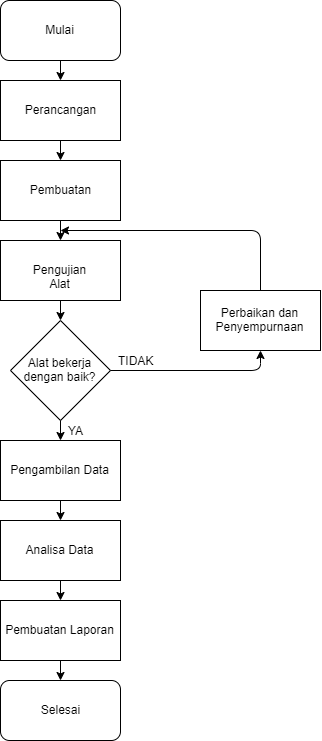
\includegraphics[width=7cm]{gambar/flowchart.png}
		\caption{\emph Flowchart Prosedur Penelitian}
	\end{figure}
	
	
\end{enumerate}

\section{Sistematika Penulisan}
Penulisan laporan kerja praktik ini dilakukan dengan mengikuti sistematika sebagai berikut :\\
\noindent
\textbf{BAB I\hspace*{0.6cm}: PENDAHULUAN}\\
\noindent
Merupakan pendahuluan dari laporan kerja praktik yang menjelaskan latar belakang, tujuan , batasan masalah dan metodologi penyusunan laporan proyek akhir\\
\noindent
\textbf{BAB II\hspace*{0.5cm}: LANDASAN TEORI}\\
\noindent
Memuat gambaran umum robot lengan, lingkup kerja (\emph workspace), konfigurasi robot lengan, perhitungan kinematika maju dan kinematika balik,pengertian dan prinsip kerja Processing IDE sebagai antarmuka robot lengan, dan prinsip kerja setiap piranti yang digunakan dalam pembuatan robot lengan, \\
\textbf{BAB III\hspace*{0.375cm}:  PERANCANGAN SISTEM}\\
\noindent
Memuat perancangan sistem secara umum, perancangan perangkat keras berupa elektronis dari robot lengan, perancangan perangkat lunak berupa pengolahan Graphical User Interface (GUI) menggunakan Processing IDE, sistem kinematika balik untuk robot lengan, dan integrasi keseluruhan program. \\
\textbf{BAB IV\hspace*{0.4cm}:  PENGUJIAN DAN ANALISA KERJA SISTEM }\\
\noindent
Memuat pengujian dan analisis kerja motor servo yang berfungsi sebagai \emph joint dari robot lengan, pengujian umpan balik melalui GUI Processing IDE serta pengujian sistem secara menyeluruh.\\
\textbf{BAB V\hspace*{0.6cm}: PENUTUP}\\
Memuat tentang kesimpulan dari perancangan , pengujian dan analisis dari sistem kerja robot, serta berisi saran – saran untuk mengembangkan penelitian kerja praktik \emph{ arm manipulator robot} SCARA lebih lanjut. \\